% =============================================================== PHYSICS ==
\section{Task 3: physics consistency}\label{sec:physics}

Task 3 has no rows. Its 15\,\% weight is earned or lost by the Task 1 answer, through the two terms of
\cref{eq:phys}. This section explains why we ended up \emph{not} imposing physics on the reconstruction, after
testing it many ways.

\subsection{The diagram term is saturated}
$\SFD$ compares the submitted per-lane flow with the triangular diagram at the submitted density. Any field whose
speed and flow are jointly plausible satisfies it. Scored against the released \code{fd\_parameters.csv}, ES4's own
speed and flow reach 0.984--0.994 on all twenty panel-splits of validation and private, with a mean absolute flow
residual of 5--15 veh/h and essentially no clipping. Exact observations score about 0.986 on the training months. A
projection of the field onto the diagram buys about +0.002 in $\Sphys$ and costs speed accuracy, so it was not used.

\subsection{The conservation term cannot be measured locally}
$\SLWR$ checks $N_{t+\Delta t}-N_t$ against boundary flows that the organizers compute from their own state. Those flows
are withheld. Our local scorer is a line-by-line equivalent of the official one: given the same boundary-flux file,
the two agree to four decimal places on eight test fields and four panels. With the flux replaced by the observed accumulation
change, it sits near the exact-answer ceiling (the organizers' perfect answer scores 0.9636 in $\Sphys$, about 0.95 in
$\SLWR$), so it is optimistic and compresses differences between methods. We therefore used it only as a
non-regression check next to $\Sstate$, never as the objective.

\subsection{Imposing physics lost every time}
We tested the most natural ways to make the reconstruction obey the kinematic-wave model \cite{lighthill1955,richards1956,treiber2013}.
Each was frozen on fitting months and scored once on held-out months (\cref{fig:physics,tab:physics}).

\begin{figure}[t]
\centering
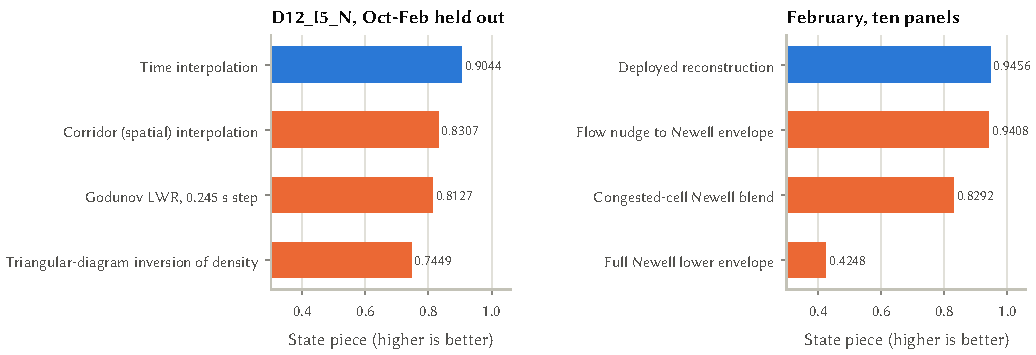
\includegraphics[width=\linewidth]{figures/fig_physics_alternatives.pdf}
\caption{Physics-based reconstructions against their controls. Left: one corridor, all October--February targets
(2,583,593 cells), where same-day interpolation is the control. Right: February on all ten panels, where the
deployed residual model is the control. Blue marks the control; TRAIN proxies.}\label{fig:physics}
\end{figure}

\begin{table}[h]
\centering\small
\caption{Physics-based reconstruction experiments. ``Piece'' is the per-cell state score of \cref{eq:state}. All
numbers are held-out TRAIN proxies; none of these variants is in a selected file.}\label{tab:physics}
\begin{tabularx}{\linewidth}{@{}X r r X@{}}
\toprule
Method & Piece & Control & Outcome \\
\midrule
Godunov LWR, 0.245 s step, 1,224 substeps per bin, released diagram, visible cells pinned \cite{godunov1959,daganzo1994} & 0.8127 & 0.9045 & congested speed RMSE 20.68 vs 8.10 km/h; gate +0.005 failed \\
Corridor (spatial) interpolation of speed and flow & 0.8307 & 0.9045 & speed RMSE 6.59 vs 2.93 km/h \\
Diagram inversion of spatially interpolated density & 0.7449 & 0.9045 & flow RMSE 104.3 vs 42.1 veh/h/lane \\
Steady flux $\min(\text{sending},\text{receiving})$ on 1,159,377 ramp-free holes & 0.8510 & 0.9074 & congested speed RMSE 18.60 vs 7.98 km/h \\
Time-interpolated speed with corridor-interpolated flow & $+$0.0037 & --- & lost on two corridors; local physics lower on seven \\
Newell lower envelope of cumulative counts \cite{newell1993} & 0.4248 & 0.9456 & speed RMSE 79.03 vs 1.60 km/h \\
Newell envelope only on congested cells & 0.8292 & 0.9456 & speed RMSE 7.36 km/h \\
Flow nudge of at most 40 veh/h/lane toward the envelope & 0.9408 & 0.9456 & physics proxy 0.700 vs 0.743; projected $-$0.0081 total \\
Congested-branch diagram flow from the interpolated speed & --- & --- & 101.4 vs 63.3 veh/h/lane on 131,696 cells, worse on all ten panels \\
Occupancy density $k=285\cdot\mathrm{occ}$ inverted through the diagram & --- & --- & below interpolation on all ten panels \\
Flow--ramp balance regression on consecutive visible pairs & --- & --- & held-out correlation 0.0009--0.0094 (bar 0.5) \\
\bottomrule
\end{tabularx}
\end{table}

\subsection{Why physics loses here}
The results share one explanation. The masked holes are short in space and time. On D12\_I5\_N, of 1,159,377
ramp-free target cells with a detector on both sides, 494,175 sit in one-link holes, 345,813 in two-link holes and
295,706 in holes of three to five links; no hole is longer than twenty links. The information about a missing cell
is mostly in its own detector a few minutes earlier and later. A fine-step solver moves a wave across the whole hole
within one five-minute bin, so its five-minute aggregate becomes a \emph{spatial} reconstruction, and spatial
reconstruction is the weaker estimator (corridor interpolation 0.831 against temporal 0.904; the solver scores 0.813).
Beyond that, incidents and capacity drops in the generator are unobserved forcing; a detector's five-minute flow is
not the cell-boundary flux of the conservation check; and the conservation signal itself is small (about 0.75\,\% of
the vehicles on a link) relative to the measurement noise.

\begin{keybox}[Insight]
In this benchmark the physics weight is best served by an accurate state, not by a physical model of the state.
The diagram term is satisfied by any accurate field, and the conservation term moved together with state accuracy in
every held-out test (for example, TS3 raised the local physics proxy by +0.0015 to +0.0018 while raising $\Sstate$).
Imposing the kinematic-wave model never beat temporal evidence on held-out months.
\end{keybox}
